\section{Individual Models} \label{sec:individual}

In this section, we describe and evaluate the individual word alignment models. All of the newly introduced models make use of the fact that NMT systems can be viewed as language models and can produce translation probabilities.

\subsection{Baseline Models} \label{subsec:baseline_models}

The first model is \fastalign{}. The second is attention-based soft word alignment extracted from MarianNMT (Attention), which was trained with guided alignment during the distillation. For the rest of this subsection, we will focus on models generating soft alignment scores (an unbounded real number corresponding to the quality of a possible alignment between two tokens) and not the alignments themselves.

\paragraph{One Token Translation ($M_1$).}

The simplest approach to get alignment scores is to compute decoder translation probability using the MT (function $m$) between every source and target token $s_i$ and $t_j$ of the source and target sentences $S$ and $T$. Single tokens are passed to the models as if they were a sentence pair. The scores are not normalized which is not an issue in this case, since the models working with these alignment scores (in \Cref{subsec:extractors}) compare output from sequences of the same length.
\begin{gather*}
\forall s_i\in S, t_j \in T: p(s_i, t_j) = m(\{s_i\}, \{t_j\})
\end{gather*}

The produced values are in a log space $(-\inf, 0]$. This approach requires $|S|\cdot |T|$ of one-token translation scorings (decoder probability of the target reference) for producing word alignments of a single sentence pair. On a CPU,\footnote{8 threads 2.3GHz Ryzen 7 3700u, no RAM to disk swapping} the models average to $2.7$s per one sentence pair alignment.

\paragraph{Source Token Dropout ($M_2$).}

A more refined approach was chosen by \citet{zintgraf2017visualizing} in which the alignment score is computed as the difference in target token probability when the source token is unknown. The exact approach is too computationally demanding (requires translation scorings with large amounts of replacement words), and therefore we use a much simpler, yet conceptually similar method by either omitting the token or replacing it with \texttt{<unk>}.\footnote{Even though subword-based MT models do not need \texttt{<unk>}, SentencePiece reserves the token \texttt{<unk>} for an unknown symbol.}
Assume $m_j(S, T)$ produces the log probability of the $j$-th target token. The sentence $S^{a/b}_i$ with an obscured token $s_i$ can be defined in two ways which leads to two versions of this model: $M_2^a$ and $M_2^b$. Output is then possibly unbounded $(-\inf,\inf)$.
\begin{gather*}
    \forall s_i \in S, t_j \in T: p(s_i, t_j) = m_j(S, T) - m_j(S^{a/b}_i, T)
\end{gather*}

\vspace{-0.8cm}

\begin{align*}
    & \text{Word deletion}\, (M_2^a): 
    & S^{a}_i = s_0, s_1, \ldots, s_{i-1}, s_{i+1}, \ldots, s_{|S|} \\
    & \text{Word substitution}\, (M_2^b):
    & S^{b}_i = s_0, s_1, \ldots, s_{i-1}, \texttt{<unk>}, s_{i+1}, \ldots, s_{|S|}
\end{align*}

This requires $|S|$ translation scorings of source and target lengths $|S|$ and $|T|$, which is comparable to $M_1$. The models average to $1.5$s per one sentence pair alignment.\footnote{ The running time is lower because in this case it is $|S|$ scorings of length $|T|$, while in $M_1$ it is $|S|\times|T|$ scorings of length $1$.}

\paragraph{Source and Target Dropout ($M_3$).}

A very similar method would be to also dropout the target token and examine how the sentence probability changes. Applying the two different ways of dropout leads to four versions of this approach. Note that in this case we compute the sentence probability (because the target word is hidden) and also do not subtract from the base sentence probability, but rather use the new sentence probability as it is. This probability should be highest if the corresponding tokens are both obscured. The probability is in log space $(-\inf, 0]$.
\vspace{0.2cm}
\begin{gather*}
    \forall s_i \in S, t_j \in T: p(s_i, t_j) = m(S^{a/b}_i , T^{a/b}_j)
\end{gather*}

\vspace{-0.8cm}

\begin{align*}
    T^a_j &= t_0, t_1, \ldots, t_{j-1}, t_{j+1}, \ldots, t_{|T|} \\
    T^b_j &= t_0, t_1, \ldots, t_{j-1}, \texttt{<unk>}, t_{j+1}, \ldots, t_{|T|}
\end{align*}

\vspace{-0.8cm}

\begin{align*}
    & \text{Word deletion, deletion ($M_3^{aa}$)} & S^a_i, T^a_j \\
    & \text{Word deletion, substitution ($M_3^{ab}$)} & S^a_i, T^b_j \\
    & \text{Word substitution, deletion ($M_3^{ba}$)} & S^b_i, T^a_j \\  
    & \text{Word substitution, substitution ($M_3^{bb}$)} & S^b_i, T^b_j
\end{align*}

This approach requires $|S|\cdot|T|$ translation scorings of source and target lengths of $|S^{a/b}|$ and $|T^{a/b}|$ for sentence $S$ translated to $T$ which is roughly $|T|$ times more than in $M_1$ and $M_2$. This makes it it the most computationally demanding approach. On average it takes $46.1$s to produce one sentence pair alignment on a CPU.

\subsection{Direct Alignment from Baseline Models} \label{subsec:extractors}

All of the models (except for \fastalign{}) are not producing the alignments themselves, but soft alignment scores $p$ for each pair of tokens $(s, t)$ in source $S$ $\times$ target $T$ sentence. The hard alignment itself can then, for example, be computed in the following ways. The parameter $\alpha$ can be estimated from the development set. The function $p$ is in general any soft alignment function (e.g. attention scores or the alignment scores from IBM model 1 EM algorithm).

\begin{enumerate}
    \item For every source token $s$ take the target tokens $t$ with the maximum score.
    \begin{gather*}
        A_1 = \bigcup_{s \in S} \{ (s, t): p(s,t) = max_r \{p(s,r) \} \}
    \end{gather*}
    
    \item For every source token $s$ take all target tokens $t$ with a high enough score (above threshold). This method is used to control the density of alignments in the work of \citet{liang2006alignment} and provides a parameter to tradeoff precision and recall.
    \begin{gather*}
        A_2^\alpha = \bigcup_{s \in S} \{(s, t): p(s,t) \ge \alpha \}
    \end{gather*}
    
    \item For every source token $s$ take any target token which has a score of at least $\alpha$ times the score of the best candidate. Special handling for negative cases in the form of a division is required to make the formula work for the whole $\mathbb{R}$. The motivation for this is $M_2$, which provides possibly unbounded alignment scores. Assume $\alpha \in (0, 1]$.
    \begin{gather*}
        A_3^\alpha = \bigcup_{s \in S} \{ (s, t): p(s,t) \ge min
        \big[ \max_r\ p(s,r) \cdot \alpha, \max_r\ p(s,r)\, /\, \alpha \big] \}
    \end{gather*}
    $A_1$ can then be expressed as $A_3^1$. Lower $alpha$ values lead to lower precision and higher recall because the algorithm includes more, less probable, alignments. A variation on this approach would be to subtract $\alpha$ instead of multiplying it. The reason for choosing multiplication is that it dynamically adapts to a wider range of intervals and bounds the parameters between $0$ and $1$. This is not the case for substraction and because of this, it would be harder to choose the right parameter. 
    
    \smallskip
    \item Similar approach is for $A_3$, but with the focus on the target side. For every target token $t$ take any source token which has a score of at least $\alpha$ times the score of the best candidate.
    \begin{gather*}
        A_4^\alpha = \bigcup_{t \in T} \{ (s, t): p(s,t) \ge min
        \big[ \max_r\ p(r,t) \cdot \alpha, \max_r\ p(r,t) / \alpha \big] \}
    \end{gather*}
    Similar reversal for $A_2$ would not make sense, because it already takes all alignment above a threshold without any consideration for the direction.
    
    \item Similarly to $M_3$ and $M_4$ it is possible to create an extractor in which instead of having a single dropout on the target side, there are a multiple of them. This way, the score would not be between the source token and the target token, but between the source token and a subset of all target tokens. Formally, this would replace the (complete) weighted graph structure with a (complete) hypergraph. Instead of just having a weight for \textit{Choose--Wählen}, there would also be a weight for \textit{\{Choose\}--\{Wählen, Sie\}}, \textit{\{Choose\}-\{Wählen, im, Popupmenü\}} etc. 
    This would, however, lead to exponential complexity in terms of target sentence length. The number of words participating in an edge would then have to be limited to the number of alignments to a single token that we can empirically expect of the given language pair. \Cref{fig:alignment_example} suggests that for English-German this could be 3.
    Upon computing the scores for all the edges in this hypergraph, a follow-up task would be to find the maximum-weight matching.
\end{enumerate}

\vspace{-0.4cm}
\paragraph{Coverage.}

The suggested greedy way of computing alignments from alignment scores is far from perfect.
In the scenario depicted in \Cref{fig:alignment_coverage}, all but the last source token (German) have been aligned with the target, each with different alignment scores. Although the model may lack any lexical knowledge of the word \textit{Übersetzung}, it should consider the prior of a word being aligned to at least one target token.

\begin{figure}[h!]
    \center
    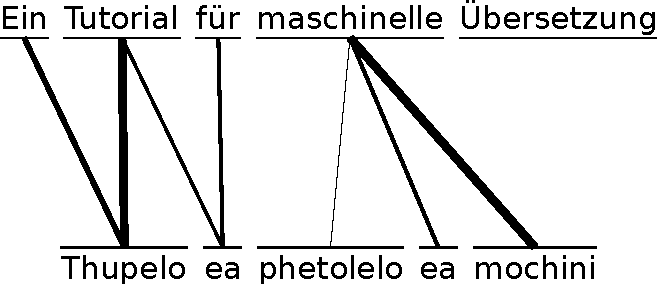
\includegraphics[width=0.5\textwidth]{alignment_coverage.pdf}
    \caption{
        Partial alignment from German (top) to Sesotho (bottom). The model has no lexical knowledge about the alignment of >>Übersetzung<<, though >>phetolelo<< is a good candidate because no other word aligned to it. Line strength corresponds to the soft alignments produced by the model.
        \label{fig:alignment_coverage}
    }
\end{figure}

In this specific case, $A_3^{0.9}$ would probably include all alignments to the word \textit{Übersetzung}, since there is no single strong candidate (assume that lines not visible depict soft alignments close to $0$). Similarly, $A_4^{0.9}$ would also include most alignments of the word \textit{Übersetzung}, including the word \textit{phetolelo}, since the alignment score with \textit{maschinelle} is weak and also close to $0$. Intersecting these two extractors $A_3^{0.9} \cap A_4^{0.9}$ would yield the correct alignment \textit{Übersetzung--phetolelo}. Other tokens would not be aligned to either of these two words because they have strong alignment scores with different tokens.

This prior may not always be desirable. For this, intersecting with $A_2^\alpha$ provides a limiting threshold. In an application where the target token is erroneous, this prevents the alignment model from aligning the two corresponding tokens.
Inducing alignment based on graph properties is examined by \citet{symmetric}, though without the presence of NMT.